\documentclass[
]{beamer}

\usepackage[english]{babel}
\usepackage[utf8]{inputenc}
\usepackage[T1]{fontenc}
\usepackage{csquotes}
\usepackage{biblatex}
\addbibresource{example.bib}
\usepackage{booktabs}
\usetheme{Pittsburgh}
\setbeamertemplate{caption}[numbered]

\title[Short Presentation Title]{Clustering BNP data with von Mises-Fisher distributions.}
%\subtitle[Short Presentation Subtitle]{Full Presentation Subtitle}
%\author[R. Speedwagon]{Robert Speedwagon\texorpdfstring{\\}{, }personal-id@mail.muni.cz}
%\institute[University Center Telč MU]{University Center Telč, Masaryk University}
\date{\today}
\subject{Presentation Subject}
\keywords{von Mises-Fisher, clustering, bionanoprobe}
\begin{document}

\begin{frame}[plain]
\maketitle
\end{frame}

\section[Short Section 1 Name]{Full Section 1 Name}
\subsection[Short Subsection 1 Name]{Full Subsection 1 Name}

% page 2
\begin{frame}{von Mises Fisher distributions}%{Subtitle}
Random vector $\boldsymbol{x}$ has a $d$-variate von Mises-Fisher (vMF) distribution if its probability density function is given by:
$$f(\boldsymbol{x}|\boldsymbol{\mu}, \kappa) = c_d(\kappa)e^{\kappa\boldsymbol{\mu}^T\mathbf{x}}$$
\begin{itemize}
  \item $\boldsymbol{x}$: random d-dimensional unit vector (i.e. $||\boldsymbol{x}|| = 1$).
  \item $\boldsymbol{\mu}$: mean direction of distribution. Also a unit vector.
  \item $\kappa$: concentration parameter.
  \begin{itemize}
    \item For $\kappa = 0$, distribution becomes uniform distribution on unit sphere. For $\kappa = \infty$, distribution becomes single point.
  \end{itemize}
  \item $c_d(\kappa)$: normalizing parameter. Given by,
  $$c_d(\kappa) = \frac{\kappa^{d/2-1}}{(2\pi)^{d/2}I_{d/2-1}(\kappa)}$$
  \begin{itemize}
      \item $I_r(\cdot)$: modified Bessel function of the first kind and order r.
  \end{itemize}
\end{itemize}
\end{frame}

% page 3
\subsection[movMF image]{Mixture of vMF distributions on the 3-sphere}
\begin{frame}{von Mises-Fisher distributions.}
\begin{figure}[h]
  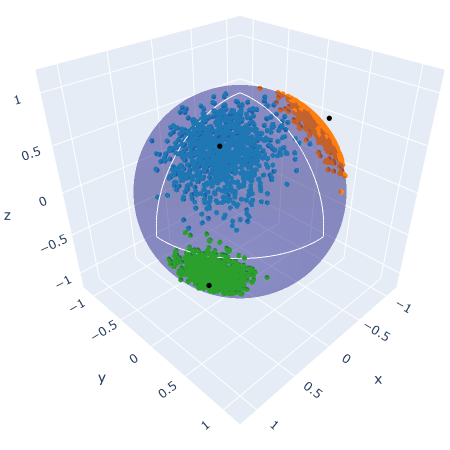
\includegraphics[width=.5\textwidth,height=.5\textheight,keepaspectratio]{vMF.png}
  \caption{Mixture of three von Mises Fisher distributions on the 3-sphere. Black spots are above $\boldsymbol{\mu}$ for each distribution. White triangle is the positive octant.
  }
\end{figure}
\end{frame}

%page 4
\subsection[Short Subsection 3 Name]{Full Subsection 3 Name}

\begin{frame}{Bionanoprobe Data.}
\begin{figure}[h]
  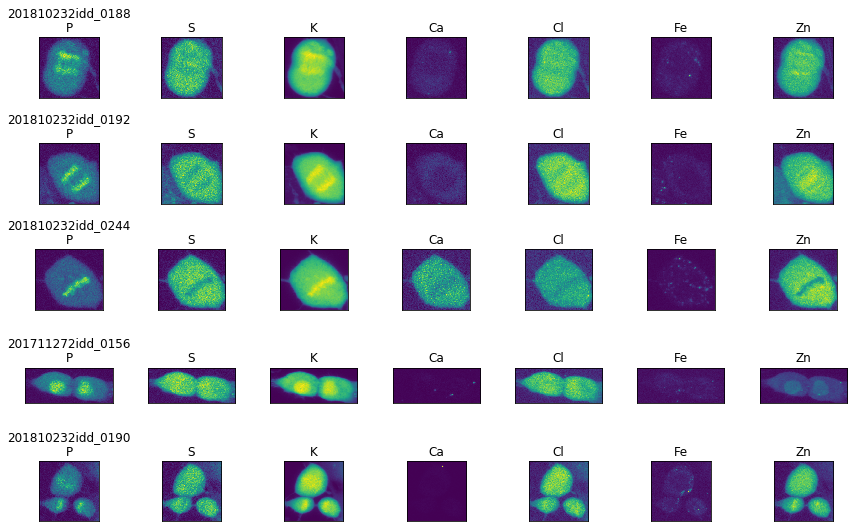
\includegraphics[width=1\textwidth,height=1\textheight,keepaspectratio]{BNP.png}
  \caption{XRF images of mouse fibroblasts.
  }
\end{figure}
\end{frame}

%page 5
\begin{frame}[Prepossessing BNP data]
For BNP data each pixel is its own d-dimensional vector $\boldsymbol{X_p}$, 
$$\boldsymbol{X_p} = (X_1, X_2, ..., X_d).$$
Where each $X_i$ corresponds to a different element. Each pixel will need to be normalized to unit length before fitting however first we must address the variance in the data.  The variance of $X_i$ for all $p$ will not necessarily be equal. vMF is a normal distribution on the hypersphere and thus assumes equal variance in each dimension so we need first scale our data. We first need to normalize this data to put it on the unit hypersphere,
$$ \boldsymbol{x_p} = \boldsymbol{X_p}/||\boldsymbol{X_p}||.$$

\end{frame}
\section{\bibname}
\begin{frame}[t, allowframebreaks]{\bibname}
\printbibliography[heading=none]
\end{frame}

\begin{frame}[plain]
\vfill
\centerline{Thank You for Your Attention!}
\vfill\vfill
\end{frame}

\end{document}
